\usetikzlibrary {automata,positioning}
% "A|BA"
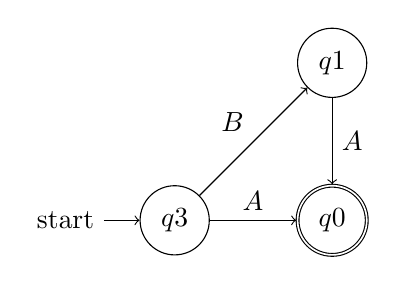
\begin{tikzpicture}[auto]
    \node[state, accepting] at (2, 0)(q0){$q0$};
    \node[state] at (2, 2)(q1){$q1$};
    \node[state, initial] at (0, 0)(q3){$q3$};
    
    \path[->]
        (q1)edge node{$A$}(q0)
        (q3)edge node{$A$}(q0)
        (q3)edge node{$B$}(q1)
        ;
\end{tikzpicture}
\captionof{figure}{After pruning with final state pruning}
\label[figure]{fig:finalStateAfter}